\documentclass[main.tex]{subfiles}
\graphicspath{{./images}}


\begin{document}
Sottoinsiemi di $ \mathbb{R} $ sono:
\begin{itemize}
        \item $ \mathbb{N} = \{0,1,2,3,\ldots\} $
        \item $ \mathbb{Z} = \{\ldots,-2,-1,0,1,2,\ldots\} $
        \item $ \mathbb{Q} = \{\frac{m}{n}: m \in \mathbb{Z} \wedge n \in \mathbb{N}^*\} $
\end{itemize}

\begin{tcolorbox}
       \begin{oss}
        In particolare $ \mathbb{Q} $ è detto \textbf{denso} ovvero  presi due qualunque punti $ x,y \in \mathbb{R} $ esiste sempre un razionale $ \mathbb{Q}  $ tra di essi.
       \end{oss} 
\end{tcolorbox}


\begin{tcolorbox}
\begin{prop}
Fondamentale proprietà di $ \mathbb{R} $ è un insieme \textbf{totalmente ordinato}.
\end{prop}
\end{tcolorbox}

\begin{lemma}
       $ \forall x,y \in \mathbb{R} $ con $ x < y $ 
\end{lemma}


\subsection{Sottoinsiemi particolari di $\mathbb{R}$}\label{sec:sottoinsiemi_particolari_di_R}

Esistono diversi tipi di intervalli, elenchiamoli per categoria


\subsubsection{Intervalli limitati}
\begin{itemize}
        \item $ (a,b) = \{x \in \mathbb{R} : x>a \wedge x<b\} $ intervallo aperto
        \item $ [a,b] = \{x \in \mathbb{R} : x\ge a \wedge x\le b\} $ intervallo chuso
        \item $ [a,b) = \{x \in \mathbb{R} : x\ge a \wedge x<b\} $ intervallo semi-aperti
        \item $ (a,b] = \{x \in \mathbb{R} : x>a \wedge x\le b\} $ itervallo semi-aperti
\end{itemize}


\subsubsection{Intervalli illimitati}
Gli intervalli illimitati sono rappresentate geometricamente da semirette

\begin{itemize}
        \item $ (a,+\infty) = \{x \in \mathbb{R} : x>a \wedge x<+\infty\} $ intervallo aperto
        \item $ [a,+\infty] = \{x \in \mathbb{R} : x\ge a \wedge x\le +\infty\} $ intervallo chuso
        \item $ [-\infty,b) = \{x \in \mathbb{R} : x\ge -\infty \wedge x<b\} $ intervallo semi-aperti
        \item $ (-\infty,b] = \{x \in \mathbb{R} : x>-\infty \wedge x\le b\} $ itervallo semi-aperti
\end{itemize}


\subsection{Dominio e Codominio}\label{sec:}
Tratteremo funzioni $ f $ che hanno un dominio $ A \subseteq \mathbb{R}$ e sottointendiamo che si parla di funzioni reali:
\begin{equation*}
        f : \mathbb{R} \to \mathbb{R}
\end{equation*}
e che quindi il dominio è il più grande insieme di definizione.

\begin{definition}
        (Funzione) Una funzione $ f:A \to R $ non è altro che una associazione \underline{univoca} di un elemento di $ A $ con uno di $ \mathbb{R} $. \par
        In particolare:
\begin{equation*}
        \forall x \in A \quad \exists! y\in\mathbb{R} : f(x) = g.
\end{equation*}
\end{definition}


\begin{tcolorbox}
\begin{prop}
       Una particolarità dei reali è che possiamo rappresentare il grafico della funzione:
\end{prop}
\end{tcolorbox}
\begin{figure}[H]
  	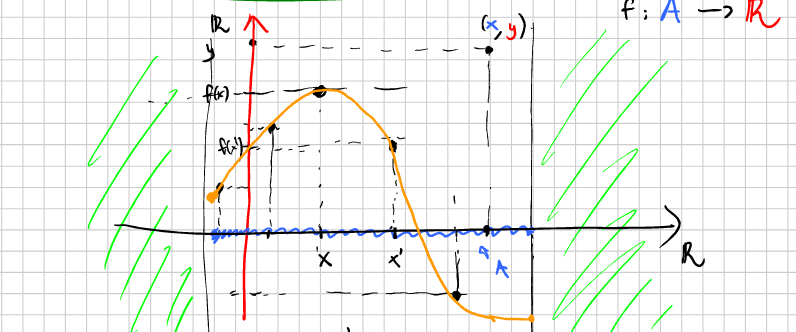
\includegraphics[width=\linewidth]{rappresentazione_grafica_reali.png}
  	\caption{}
        \label{fig:rappresentazione_grafica_reali.png}
\end{figure}

Come la retta rappresenta l'insieme $ \mathbb{R} $ il piano rappresenta l'insieme:
\begin{equation*}
        \boxed{\mathbb{R}\times\mathbb{R} = \{(x,y): x\in \mathbb{R}, y \in \mathbb{R}\}}
\end{equation*}
Il grafico di $ f $ non è altro che:
\begin{equation*}
        \boxed{graph(f) = \{(x, f(x)) : x \in A = dom(f)\}\le \mathbb{R}^2}
\end{equation*}

\begin{tcolorbox}
\begin{oss}
        Data una curva $ M \subseteq \mathbb{R}^2 $, essa è grafico di una funzione solo se $ \forall x \in \mathbb{R}$ esiste al più un punto $ y $ tale che $ (x,y) \in M $, cioè $ M $ intergetta le rette verticali al più di un punto\par
        Immaginiamo per esempio le parabole nella forma $ ax^2 + bx + c $.
\end{oss}
\end{tcolorbox}
Ciao come va? 
\definecolor{c1314613}{HTML}{000000}
\begin{align*}
\begin{tikzpicture}
\begin{axis}[
        legend pos=outer north east,
        title=test,
        axis lines = middle,
        xlabel = $x$,
        ylabel = $y$,
        domain=-250:250,
        variable = t,
        trig format plots = rad,
]
\addplot [
        samples=70,
        color=c1314613
]
        {15.81889253018077 -0.788186605035093 * x ^ 1 + 0.012375069065787742 * x ^ 2};
\addlegendentry{$y=15.8 -0.788x + 0.012x ^ 2$}
\addplot+[sharp plot]
coordinates {
        (-67,126) (-38,71) (-25,43) (-7,16) (-6,8) (18,10) (59,17) (117,105) (135,124) 
};
\end{axis}
\end{tikzpicture}
\end{align*}

\end{document}        
